\chapter{Collision Probability Method}
\label{lec:cpm}

In the last lecture, we discussed the integral transport equation, derived its form in slab geometry, and provided a simple numerical approach based on Neumann iteration and numerical quadrature for solving homogeneous slab problems.  In this lecture, we discuss the rather versatile \textit{collision probability method} in slab geometry, though the method is certainly applicable to higher dimensions.  We finish by providing a simple code that serves as the basis for several exercises.

\section*{Collision Probabilities}

Recall Eq. \ref{eq:integralphislab}, the integral equation in slab geometry:
\begin{equation}
 \phi(x) =  \int^{\infty}_{-\infty} dx'\frac{1}{2} E_1(\tau(x,x'))Q(x') \, ,   
 \tag{\ref{eq:integralphislab}}     
\end{equation}
where the emission density $Q$ contains any external and scattering sources, all assumed to be isotropic.  Suppose we apply this equation to a finite slab of length $L$ with vacuum boundaries, much as we did toward the end of Lecture \ref{lec:integral}, or
\begin{equation}
 \phi(x) = \int^L_0  dx' \frac{1}{2} E_1(\tau(x,x')) Q(x') \, .
 \label{eq:cpmphi}
\end{equation}


Let us assume the slab can be divided into a number of regions in which all cross-sections and external sources uniform, as in Figure \ref{fig:slab_spatial}.  
\begin{figure}[t] 
    \centering
    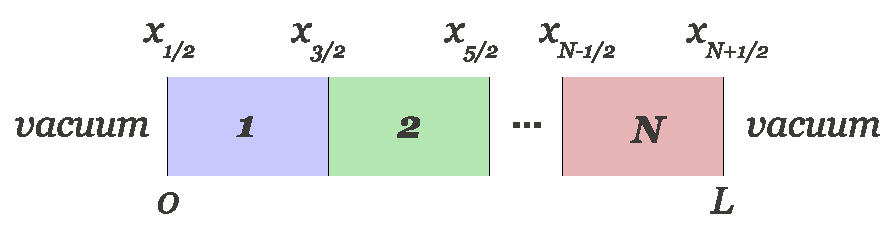
\includegraphics[keepaspectratio, width = 4.0 in]{images/cpmslab}
    \caption{Slab discretization for CPM.}
    \label{fig:slab_spatial}
\end{figure}
Within a region $i$ spanning $x_{i-1/2}$ to $x_{i+1/2}$, we define an average flux
\begin{equation}
 \phi(x_i) = \phi_i \equiv \frac{1}{\Delta_i} \int^{x_{i+1/2}}_{x_{i-1/2}} \phi(x) dx \, ,
 \label{eq:phiigeneral}
\end{equation}
where $\Delta_i \equiv x_{i+1/2}-x_{i-1/2}$.  Substituting the expression for $\phi$ in Eq. \ref{eq:cpmphi} into Eq. \ref{eq:phiigeneral} yields
\begin{equation}
 \phi_i = \frac{1}{\Delta_i} \int^{x_{i+1/2}}_{x_{i-1/2}} dx \int^L_0  dx' \frac{1}{2} E_1(\tau(x,x')) Q(x') \, .
 \label{eq:phii}
\end{equation}

% We define an average emission density $Q$ within a cell as
% \begin{equation}
%  Q_i \equiv \frac{1}{\Delta_i} \int^{x_{i+1/2}}_{x_{i-1/2}} Q(x) dx \, ,
%  \label{eq:constantq}
% \end{equation}
% which can b
If we assume the flux within the cell is its average (a constant), then the emission density is also constant, and we find
\begin{equation}
  \int^L_0  dx' \frac{1}{2} E_1(\tau(x,x')) Q(x')  dx \approx \sum^N_{i=1}  Q_i \int^{x_{i+1/2}}_{x_{i-1/2}} dx' \frac{1}{2} E_1(\tau(x,x'))  \, .
\end{equation}
Substituting this into Eq. \ref{eq:phii} (and being mindful of primes) yields
\begin{equation}
\begin{split}
 \phi_i &= \frac{1}{\Delta_i} \int^{x_{i+1/2}}_{x_{i-1/2}} dx \Bigg ( \sum^N_{i'=1} Q_{i'} \int^{x_{i'+1/2}}_{x_{i'-1/2}} dx' \frac{1}{2}E_1(\tau(x,x')) \Bigg )  \\
        &= \frac{1}{\Delta_i}  \sum^N_{i'=1} Q_{i'} \int^{x_{i+1/2}}_{x_{i-1/2}} dx \int^{x_{i'+1/2}}_{x_{i'-1/2}} dx' \frac{1}{2} E_1(\tau(x,x')) 
\end{split}
\label{eq:phii2}
\end{equation}

The collision probability method (as the name might imply) actually deals in terms of reactions rates rather than just the flux.  If we multiply both sides of  \ref{eq:phii2} by $\Sigma_i \Delta_i$, where $\Sigma_i$ is the total cross-section in region $i$, we get an equation for $\phi_i \Sigma_i \Delta_i$, the total collision rate within region $i$.  This equation is
\begin{equation}
\begin{split}
 \phi_i \Sigma_i \Delta_i &= \Sigma_{i} \sum^N_{i'=1} Q_{i'} \int^{x_{i+1/2}}_{x_{i-1/2}} dx \int^{x_{i'+1/2}}_{x_{i'-1/2}} dx' \frac{1}{2} E_1(\tau(x,x'))   \\
        &=  \sum^N_{i'=1} Q_{i'} \Delta_{i'} \frac{\Sigma_{i}}{\Delta_{i'}} \int^{x_{i+1/2}}_{x_{i-1/2}} dx \int^{x_{i'+1/2}}_{x_{i'-1/2}} dx' \frac{1}{2} E_1(\tau(x,x'))  \\
        &= \sum^N_{i'=1} Q_{i'} \Delta_{i'} P_{ii'} \, ,
\end{split}
\label{eq:cpmeqs}
\end{equation}
where 
\begin{equation}
\begin{split}
 P_{ii'} \equiv\frac{\Sigma_{i}}{\Delta_{i'}} \int^{x_{i+1/2}}_{x_{i-1/2}} dx \int^{x_{i'+1/2}}_{x_{i'-1/2}} dx' \frac{1}{2} E_1(\tau(x,x')) \, 
\end{split}
\label{eq:firstflightcollprob}
\end{equation}
is the \textit{first-flight collision probability}.  Notice we rearranged terms such that $P_{ii'}$ is unitless.  Moreover, $P_{ii'}$ can be interpreted as the probability that a neutron born uniformly and isotropically in a region $i'$ makes its first collision in region $i$.

\section*{Solving the Equations}
Eq. \ref{eq:cpmeqs} provides a set of equation for the scalar flux (or rather, the collision rates) in terms of the region emission densities $Q_i$ and collision probabilities $P_{ii'}$.  In our case of slab geometry, we can compute the collision probabilities analytically.  We simply list the results, leaving the derivations as exercises:
\begin{equation}
\begin{split}
 P_{ii}  &= 1 - \frac{1}{2\Sigma_i \Delta_i} \Big ( 1-2E_3(\Sigma_i \Delta_i) \Big ) \\
 P_{ii'} &= \frac{1}{2\Sigma_i' \Delta_i'} \Big ( E_3(\tau_{ii'}) - E_3(\tau_{ii'}+\Delta_i \Sigma_i) - E_3( \tau_{ii'} + \Delta_{i'} \Sigma_{i'}) \\
         &+ E_3(\tau_{ii'} + \Delta_i \Sigma_i + \Delta_{i'} \Sigma_{i'} ) \Big ) \, , \,\,\, i \neq i' \, ,
\end{split}
\end{equation}
where
\begin{equation}
 \tau_{ii'} \equiv \begin{cases} \tau( x_{i+1/2}, x_{i'-1/2} )   &   i' > i  \\
                            \tau( x_{i'+1/2}, x_{i-1/2} )   &   i' < i  \\
 \end{cases} \, .
\end{equation}

So how do we solve the equations once we have the $P_{ii'}$?  We have a system of equations of the form
\begin{equation}
 \Delta_i \Sigma_i \phi_i = \sum^N_{i'=1} ( \Delta_{i'} \Sigma_{si'}\phi_{i'} + S_{i'}\Delta_{i'})P_{ii'} \, .
\end{equation}
If we rearrange terms, bringing all $\phi$'s to the left hand side, we can write for $i=1$
\begin{equation}
 \Delta_1 ( \Sigma_1 - P_{11}\Sigma_{s1} ) \phi_1 - P_{12} \Delta_2 \Sigma_{s2} \phi_2 + \ldots =  S_{1}\Delta_{1}P_{11} + S_{2} \Delta_2 P_{12} + \ldots 
\end{equation}
If we define $f_i = \Delta_i \Sigma_i \phi_i$ and $s_i = \sum_{i'} S_{i'}\Delta_{i'}P_{ii'}$, this becomes
\begin{equation}
\Big ( 1-\frac{\Sigma_{s1}}{\Sigma_{1}}P_{11} \Big ) f_1 + \Big ( -\frac{\Sigma_{s2}}{\Sigma_2}P_{12} \Big ) f_2 + \ldots =  s_i \, .
\end{equation}
Generalizing to matrix form, we have
\begin{equation}
  \mathbf{ H } \mathbf{ f } = \mathbf{ s } \, ,
  \label{eq:cpmmatrix}
\end{equation}
where
\begin{equation}
 \mathbf{H} = 	\left
	[\begin{array}{cccccc}
    1-\frac{\Sigma_{s1}}{\Sigma_{1}}P_{11} & -\frac{\Sigma_{s2}}{\Sigma_2}P_{12} &  -\frac{\Sigma_{s3}}{\Sigma_2}P_{13} & \cdots & & \\
     -\frac{\Sigma_{s1}}{\Sigma_{1}}P_{21} &1-\frac{\Sigma_{s2}}{\Sigma_2}P_{22} &  -\frac{\Sigma_{s3}}{\Sigma_2}P_{23} & \cdots & & \\
	    &       &        & \ddots    &    &      \\
	\end{array} 
	\right ] \, .
\end{equation}

For a purely absorbing case, Eq. \ref{eq:cpmmatrix} is quite simple, as $\mathbf{H}$ reduces to the identity matrix.  Suppose we have a four region problem, with a source in just the third region.  The resulting set of linear equations is simply
\begin{equation}
  \mathbf{H} = 	\left
	[\begin{array}{cccc}
        1 & 0 & 0 & 0 \\
        0 & 1 & 0 & 0 \\ 
        0 & 0 & 1 & 0 \\
        0 & 0 & 0 & 1
	\end{array} 
	\right ] 
	\left
	[\begin{array}{c}
	  \Delta_1 \Sigma_1 \phi_1    \\
	  \Delta_2 \Sigma_2 \phi_2    \\
	  \Delta_3 \Sigma_3 \phi_3    \\
	  \Delta_4 \Sigma_4 \phi_4    \\
	\end{array} 
	\right ] =
	\left
	[\begin{array}{c}
	  S_3 P_{13} \Delta_3       \\
	  S_3 P_{23} \Delta_3       \\
	  S_3 P_{33} \Delta_3       \\
	  S_3 P_{43} \Delta_3       \\
	\end{array} 
	\right ] \, ,
\end{equation}
the solution of which is simply $\phi_1 = (S_3 P_{13} \Delta_3)/(\Delta_1 \Sigma_1)$ and so forth.

\section*{Benefits and Limitations}

Eq. \ref{eq:cpmmatrix} is powerful (as are integral methods in general) in that no angular approximation in the flux are made.  However, the sources and scattering are assumed to be isotropic, which does limit to an extent the accuracy in angle.

Furthermore, the collision probability suffers from two rather significant deficiencies.  First, the matrix $\mathbf{H}$ is in general a dense matrix.  Hence, for large problems, the memory requirements are significant.  Furthermore, the flat flux approximation within a region is only first-order accurate (meaning errors are proportional to $\Delta_i$).

\section*{More Advanced Aspects}

In the discussion above, we considered only vacuum conditions.  The collision probability method has been most heavily used in lattice physics calculations, where the domain is often represented as an infinite array of identical unit cells via periodic boundary conditions.  

To derive these conditions would be beyond our intended scope, but the reader might conclude the derivation would, theoretically, involve infinite sums over $P_{ii'}$, and this is indeed the case.  The interested reader is encouraged to read Section 3.8.3 of Hebert \cite{hebert2009arp} for discussion of a suitable numerical approach.

\section*{A Simple Code}

Here, we provide a simple code for computing the scalar flux in a slab consisting of several regions of uniform composition, given in Listing \ref{list:cpm}.  The fundamental components of the code are just those that compute $\tau$ and $P_{ii'}$ and should be readily understood.  As in the Neumann iteration code of the last lecture, MATLAB's built in symbolic function for the exponential integrals is used.  This is very slow, and so the student is encouraged to find efficient and accurate numerical techniques to evaluate these functions.  

\lstset{language=Octave,caption=Solution of Slab Problem via CPM, label=list:cpm, morecomment=[l]{\%}}
\lstinputlisting{code/cpm.m}

\section*{Further Reading}

This lecture has largely followed Section 5-3 of Lewis and Miller \cite{lewis1993cmn}.  There, the student will find some more details regarding periodic conditions for slab geometry as well as some information regarding a 2-d implementation of CPM in later sections.  Hebert \cite{hebert2009arp} also discusses CPM in several geometries and provides sample code relevant for both slab and a 2-d pin cell problems.

\begin{exercises}
  \item \textbf{CPM and Scattering}. Use the CPM code to repeat Exercise 6 of Lecture \ref{lec:integral}.  Does increase scattering have any effect on the computational time?  Why or why not?

  \item \textbf{Source Iteration}. In our (relatively standard) formulation of the collision probability method, we end up with a dense matrix $\mathbf{H}$.  Reformulate the approach such that the scattering term is \textit{not} brought to the left hand side.  In this case, $\mathbf{H}$ is just the identity.  However, the right hand side now contains an additional scattering source contribution, which depends on the (unknown) fluxes.  Develop an approach such that the flux is initially guessed, the right hand side is formed, new fluxes are computed, and the right hand side is updated, yielding an iterative process called \textit{source iteration}.  

  \item \textbf{CPM with Source Iteration}. Implement the \textit{source iteration} you developed in the last exercise in the given CPM code.  Repeat Exercise 6 from Lecture \ref{lec:integral}, using a stopping criterion of 
  \begin{equation*}
   \frac{|\phi^n_i-\phi^{n-1}_i|}{\phi^{n-1}_i} < \epsilon = 1\times10^{-6} \, \, \, \, \, \, \forall \, i \, ,
  \end{equation*}
  where $n$ is the iteration index.  Comparing to Exercise 1, is there any benefit to using source iteration in place of solving a dense matrix system directly?  If not for this particular problem, underwhat conditions would you expect source iteration to be better?

  \item \textbf{Understanding Periodic Conditions}. Read Section 3.8.3 of Hebert and provide a short synopsis of period conditions can be treated in slab geometry.

  \item \textbf{Implementing Periodic Conditions}. Implement periodic conditions in the given CPM code, following the method described by Hebert.


\end{exercises}
